\documentclass{beamer}
\usepackage{pgfplots}

\usepgfplotslibrary{dateplot}
\usetheme{m}

\title{Brave New OCaml World}
\author{Marek Kubica}
\institute{Lambda Days}
\date{25.2.2015}

\titlegraphic{\includegraphics[width=\linewidth]{colour-transparent-logo}}
\pgfplotsset{compat=1.10}
%\pgfplotsset{compat=1.11}

% Not sure we even want a logo
%\logo{\includegraphics[width=1cm]{colour-transparent-icon}}

\renewcommand{\itemBullet}{\hbox{\vrule width 1ex height 1ex}}
\setsansfont[BoldFont={Lato}]{Lato Light}
\newfontfamily\exclaim{Lato Black}

\newfontfamily\ExtraLight{Lato Light}
\newfontfamily\Light{Lato Light}
\newfontfamily\Medium{Lato Medium}
\begin{document}

\maketitle

\begin{frame}{Who am I even?}
  \begin{columns}[c]
    \column{.5\textwidth}
      
\includegraphics[height=0.8\textheight]{programmers}
    \column{.5\textwidth}
      \begin{itemize}
        \item From Technische Universität München
        \item Introduction to Programming lecture with OCaml
        \item Then, Bachelor Thesis: OCaml
        \item Now, Master Thesis: OCaml
      \end{itemize}
  \end{columns}
\end{frame}

\begin{frame}{}
  \center
  \fontsize{70}{70} \exclaim Why?
\end{frame}

\begin{frame}{Quick feature list}
  \begin{itemize}
    \item Static Hindley-Milner type system with inference
    \item Fast
    \item Strict
    \item Quick native and byte code compilers
    \item Wide variety of platforms supported
    \item One single language (not 70 language extensions)
    \item Macro system
    \item Good backwards compatibility
  \end{itemize}
\end{frame}

\begin{frame}{But it's unpopular!}
  \#38 language on GitHub

  % logos
  
\includegraphics[height=1cm]{facebook}
  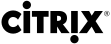
\includegraphics[height=1cm]{citrix}
  
\includegraphics[height=1cm]{janestreet}
  
\includegraphics[height=1cm]{esper}
  
\includegraphics[height=1cm]{galois}
  \includegraphics[height=1cm]{shiro}
  
\includegraphics[height=1cm]{ds}
  
\includegraphics[height=1cm]{issuu}
  % TODO
\end{frame}

\begin{frame}{OPAM stats: packages}
  \begin{tikzpicture}
    \begin{axis}[
      xlabel=Time,
      ylabel=Packages,
      ymin=0,
      xmin=2012-08-21,
      %axis x line=bottom,
      %axis y line=left,
      enlargelimits=false,
      %enlarge x limits=upper,
      enlarge y limits=upper,
      grid=major,
      date coordinates in=x,
      xticklabel={\month.\year},
      xticklabel style={rotate=90},
      legend entries={Total, Unique},
      legend style={legend pos=north west},
      width=\textwidth,
      height=.8\textheight,
      ytick={0,500,...,3500},
      ]

      \addplot [color=red,fill=red!50, fill opacity=0.8] table {packages.csv}\closedcycle;
      \addplot [color=blue,fill=blue!50, fill opacity=0.6] table {unique-packages.csv}\closedcycle;
    \end{axis}
  \end{tikzpicture}
\end{frame}

\begin{frame}{OPAM stats: OPAM repository contributors}
  \begin{tikzpicture}
    \begin{axis}[
      xlabel=Time,
      ylabel=Contributors,
      ymin=0,
      %axis x line=bottom,
      %axis y line=left,
      enlargelimits=false,
      %enlarge x limits=upper,
      enlarge y limits={value=0.15,upper},
      grid=major,
      date coordinates in=x,
      xticklabel={\month.\year},
      xticklabel style={rotate=90},
      width=\textwidth,
      height=.8\textheight,
      try min ticks=9,
      ytick={0,50,...,300},
      fill opacity=0.8,
      ]

      \addplot [color=blue,fill=blue!50] table {contributors.csv}\closedcycle;
    \end{axis}
  \end{tikzpicture}
\end{frame}

\section{Learning}

\begin{frame}{Real World OCaml}
  \begin{columns}[c]
    \column{.5\textwidth}
      
\includegraphics[height=0.8\textheight]{rwo}
    \column{.5\textwidth}
      \begin{itemize}
        \item The best OCaml book ever published
        \item For more experienced developers
        \item Broad amount of topics covered: functional programming
          object orientation, runtim
        \item Uses Jane Street's Core Standard library
        \item Freely available online
      \end{itemize}
  \end{columns}
\end{frame}

\begin{frame}{OCaml from the very beginning}
  \begin{columns}[c]
    \column{.5\textwidth}
      
\includegraphics[height=0.8\textheight]{very-beginning}
    \column{.5\textwidth}
      \begin{itemize}
        \item Introduction into functional programming
        \item More geared towards novices
        \item A bit like "The Little Schemer"
        \item Companion book "More OCaml" available
      \end{itemize}
  \end{columns}
\end{frame}

\section{Editing}

\begin{frame}{Editor selection}
  \begin{columns}[t]
    \column{.5\textwidth}
    \begin{block}{Emacs}
      \begin{itemize}
        \item ocaml-mode
        \item Tuareg
      \end{itemize}
    \end{block}
    \begin{block}{Vim}
      \begin{itemize}
        \item OCaml syntax
        \item Operator replacement
      \end{itemize}
    \end{block}
    \begin{block}{Eclipse}
      OCaml Development Tools
    \end{block}
    \column{.5\textwidth}
    \begin{block}{Merlin}
      Helper that \emph{understands} OCaml code. Offers \emph{sensible}
      completion, type inference, renaming, definition location.
      \begin{itemize}
        \item Vim
        \item Emacs
        \item Sublime Text
      \end{itemize}
    \end{block}
  \end{columns}
\end{frame}

\section{Building}

\subsection{OASIS}

\section{Testing}

\section{Distributing}

\subsection{OPAM}

\section{What's missing}

\begin{frame}{Questions?}
  \centering
  
\includegraphics[height=.85\textheight]{camel}
\end{frame}

\end{document}
